\documentclass{article}

\usepackage{Vor2018skil}

\title{Tölvunarfræði 2, \semester \\ Skilaverkefni 10}
\author{}

\begin{document}
\maketitle
\hypersetup{pdftitle={Tölvunarfræði 2 - Skilaverkefni 10}}

Skila skal þessum verkefnum á \href{https://gradescope.com/courses/14122}{Gradescope}.

Þegar forriti er skilað inn til yfirferðar er mikilvægt að láta \textbf{niðurstöðurnar fylgja}. Öllum forritskóða skal skila framsettum með jafnbilaletri. Hann þarf að vera afritanlegur úr .pdf skjalinu. Vönduð framsetning og læsilegur kóði er hluti af verkefninu.

\question
Net eins og þau eru útfærð í \texttt{Graph.java} eru fjölnet \eng{multigraphs}. Sú útfærsla leyfir meira en einn legg á milli hverra tveggja hnúta og lykkjur \eng{loops}, leggi með báða enda tengda við sama hnút.

Algengt er að takmarka net svo að þau hafi engar lykkjur og að hámarki einn legg á milli hverra tveggja hnúta. Slík net eru kölluð einföld net \eng{simple graphs}.

Skrifið klasann \texttt{SimpleGraph.java} sem erfir frá \texttt{Graph.java} en kemur í veg fyrir að endurteknum leggjum eða lykkjum sé bætt við netið. Það er gert með því að fækka smiðunum og láta \texttt{addEdge} aðferðina valda \texttt{IllegalArgumentException} þegar slíkt er reynt.

\href{https://raw.githubusercontent.com/Ernir/kennsluefni/master/T2/Code/w11/SimpleGraph.java}{Beinagrind} er gefin ásamt \href{https://raw.githubusercontent.com/Ernir/kennsluefni/master/T2/Code/w11/tinyG.txt}{gagnaskrá}. Ekki breyta \texttt{main} aðferðinni eða haus \texttt{addEdge}. 

\question
Frávik\footnote{þýðing kennara, aðrar þýðingar velkomnar} \eng{eccentricity} hnúts er lengd stystu leiðar frá hnútnum til þess hnúts sem lengst er frá honum. Þvermál \eng{diameter} nets er mesta frávik hnúta netsins. Radíus \eng{radius} nets er minnsta frávik hnúta netsins. Miðhnútur \eng{central point} nets er hnútur með frávik sem er jafnt radíus netsins.

Skrifið forrit sem reiknar þessa eiginleika samkvæmt eftirfarandi skilum:

\begin{center}
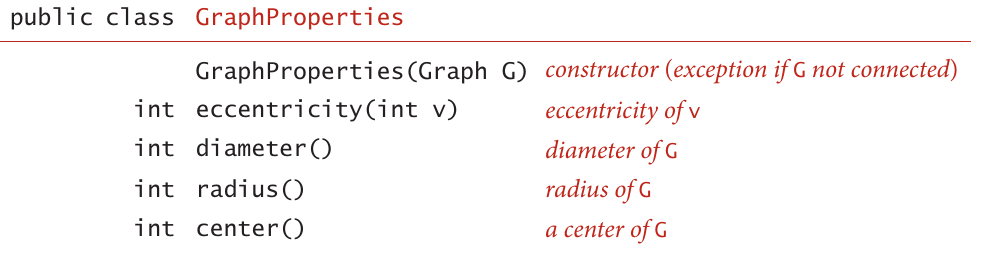
\includegraphics[width=\textwidth]{graph-properties}
\end{center}

\href{https://raw.githubusercontent.com/Ernir/kennsluefni/master/T2/Code/w11/GraphProperties.java}{Beinagrind} ásamt gagnaskránni \href{https://raw.githubusercontent.com/Ernir/kennsluefni/master/T2/Code/w11/routes.txt}{routes.txt} er gefin. Ekki breyta \texttt{main} aðferðinni eða haus aðferðanna sem þarf að útfæra. Þegar forritið er keyrt er niðurstaðan eftirfarandi:

\begin{verbatim}
Done reading routes.txt
Eiginleikar leiðanetsins:

Þvermál: 4
Radíus:  2
Miðja:   ORD

 Völlur frávik 
===============
   JFK     3   
   MCO     4   
   ORD     2   
   DEN     3   
   HOU     3   
   DFW     2   
   PHX     3   
   ATL     3   
   LAX     4   
   LAS     4  
\end{verbatim}

\question
Það að ákvarða Bacon-tölu ýmissa leikara er vinsæll samkvæmisleikur meðal netafræðinga. Þegar ákvarða skal Bacon tölu fyrir leikara fær leikarinn Kevin Bacon Bacon-töluna 0, leikari sem leikið hefur í mynd með Kevin Bacon fær Bacon-töluna 1, leikari sem leikið hefur í mynd með leikara sem hefur leikið í mynd með Kevin Bacon fær Bacon-töluna 2 (nema viðkomandi leikari eigi rétt á lægri Bacon-tölu) og svo koll af kolli. Sé ekki mögulegt að finna leið á milli leikarans og Kevins Bacons í gegnum sameiginleg leikverk er Bacon-tala viðkomandi leikara óskilgreind.

Skrifið forrit sem leitar í gegnum \href{https://raw.githubusercontent.com/Ernir/kennsluefni/master/T2/Code/w11/movies.txt}{movies.txt}, finnur Bacon-tölu allra leikaranna sem þar eru taldir upp og skrifar út fjölda leikara sem eru með hverja tölu, á eftirfarandi sniði:

\begin{verbatim}
0: 1
1: 1324
2: 70717
3: 40862
4: 1591
5: 125
Óskilgreint: 621
\end{verbatim}

Sem hér (eðlilega) segir okkur að nákvæmlega einn leikari hafi Bacon-töluna 0, 1324 leikarar Bacon-töluna 1, og svo framvegis.

Nota má hugmyndir í \href{https://github.com/Ernir/kennsluefni/tree/master/T2/Code/w11/SixDegrees.java}{SixDegrees.java}.

\vfill

\includegraphics[width=0.5\linewidth]{hi-von-logo}
\end{document}